\section{Results}
\label{sec:results}
Our primary system, \textbf{Gemma-4-31B}, scores \textbf{0.459}
relation-averaged macro-F\textsubscript{1} (\textbf{0.490} micro) on
validation---versus $0.175$/$0.203$ (empty), $0.273$/$0.284$ (official baseline),
and $0.416$/$0.447$ for the smaller Qwen2.5-14B. Figure~\ref{fig:bars} and
Table~\ref{tab:results} give the per-relation picture. Gemma-4-31B \emph{beats
the official baseline on all six relations} and the 14B on four of six; the
gains are largest on \textsc{companyTradesAtStockExchange} ($0.62\!\to\!0.72$)
and \textsc{hasCapacity} ($0.09\!\to\!0.17$, nearly doubled), while
\textsc{countryLandBordersCountry} reaches $0.953$. It ties the 14B on
\textsc{hasArea} and trails only on \textsc{personHasCityOfDeath}
($0.46$ vs.\ $0.48$)---the one relation where the single-sample 30B forgoes the
abstention voting the 14B uses. Strikingly, the 30B attains its lead
\emph{without} self-consistency or abstention, indicating that model scale
outweighs those decode-time mechanisms at this budget.

\begin{figure}[t]
\centering
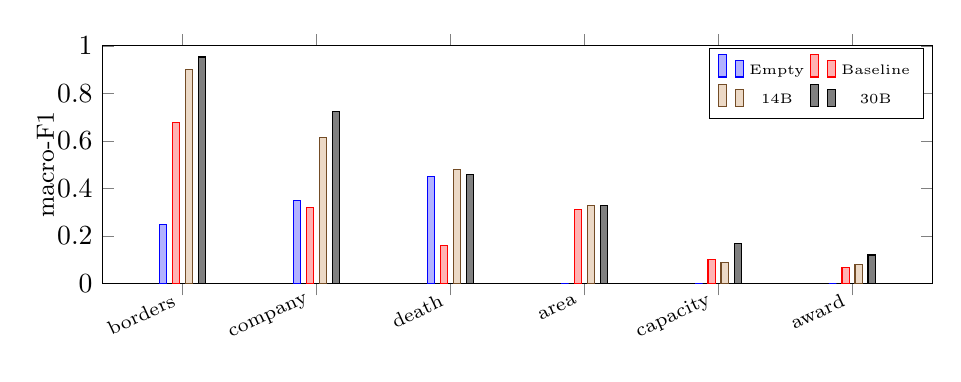
\begin{tikzpicture}
\begin{axis}[ybar,width=\columnwidth,height=4.6cm,bar width=2.7pt,
 symbolic x coords={borders,company,death,area,capacity,award},
 xtick=data,ymin=0,ymax=1,ylabel={\small macro-F1},
 ylabel style={yshift=-2mm}, legend style={font=\tiny,at={(0.99,0.99)},anchor=north east,legend columns=2},
 enlarge x limits=0.12, x tick label style={font=\scriptsize,rotate=25,anchor=east}]
\addplot coordinates {(borders,0.25)(company,0.35)(death,0.45)(area,0)(capacity,0)(award,0)};
\addplot coordinates {(borders,0.679)(company,0.32)(death,0.16)(area,0.31)(capacity,0.10)(award,0.069)};
\addplot coordinates {(borders,0.90)(company,0.616)(death,0.48)(area,0.33)(capacity,0.09)(award,0.081)};
\addplot coordinates {(borders,0.953)(company,0.722)(death,0.46)(area,0.33)(capacity,0.17)(award,0.12)};
\legend{Empty,Baseline,14B,30B}
\end{axis}
\end{tikzpicture}
\caption{Per-relation validation macro-F\textsubscript{1}: predict-nothing
baseline, official baseline, Qwen2.5-14B, and Gemma-4-31B (30B). The 30B beats
the official baseline on all six relations.}
\label{fig:bars}
\end{figure}

\begin{table}[t]
\centering\footnotesize
\setlength{\tabcolsep}{3.5pt}
\begin{tabular}{lrrrr}
\toprule
Relation & Empty & Base & 14B & \textbf{30B} \\
\midrule
countryLandBorders  & 0.250 & 0.679 & 0.900 & \textbf{0.953} \\
companyTrades       & 0.350 & 0.320 & 0.616 & \textbf{0.722} \\
personCityOfDeath   & 0.450 & 0.160 & \textbf{0.480} & 0.460 \\
hasArea             & 0.000 & 0.310 & 0.330 & 0.330 \\
hasCapacity         & 0.000 & 0.100 & 0.090 & \textbf{0.170} \\
awardWonBy          & 0.000 & 0.069 & 0.081 & \textbf{0.120} \\
\midrule
Avg.\ of relations  & 0.175 & 0.273 & 0.416 & \textbf{0.459} \\
Micro (all inst.)   & 0.203 & 0.284 & 0.447 & \textbf{0.490} \\
\bottomrule
\end{tabular}
\caption{Validation macro-F\textsubscript{1} by model. ``Empty'' is the measured
predict-nothing baseline, ``Base'' the official baseline; \textbf{30B} is our
primary Gemma-4-31B system, 14B is Qwen2.5-14B. Best per row in bold.
Gemma-4-31B beats the official baseline on \emph{all six} relations.}
\label{tab:results}
\end{table}
